\documentclass[a4paper,12pt]{scrartcl}
\usepackage{amsmath}
\usepackage{circuitikz}
\usetikzlibrary{shapes.misc} 
%\usepackage{showframe}
\begin{document}

\title{Activité Experimentale 20 - Les Cellules Photovoltaïques}
\author{Elliot Jullier}
\date{\today}
\maketitle

\pagenumbering{arabic}
\section{Fonctionnement de la Cellule Photovoltaïque}
\subsubsection*{1.1 Pourquoi la cathode (2) est une grille et non une plaque comme l'anode (5)?}


La cathode est une grille car elle doit laisser passer les photons qui sont 
la source d'énergie électrique qui est ensuite convertie en énergie électrique.
\subsubsection*{1.2 Pourquoi utiliser des semi-conducteurs dopés dans les couches (3) et (4)?}

Dans la couche dite `couche $n$', le phosphore a 5 électrons de valence, 
alors que le silicium a 4 électrons de valence. L'atome de phosphore a un électron de plus que le materiel qui l'entoure
et sera considéré comme portant une charge négative. 
Au contraire, dans la `couche $p$', les atomes de bore ont 3 électrons et  cette lacune
peut donc être assimilée à une charge positive. Quand on met les deux couches ensemble, il y a 
une couche positive et une couche négative ce qui crée un champ électrique entre les deux couches.

\subsubsection*{1.3 Soit l'énergie transportée par un photon et $\Delta E$ le "gap" de la bande interdite du silicium.
Quelle inégalité doit exister entre l'énergie du photon et $\Delta E$ pour qu'un photon arrache un 
électron à un atome de silicium?}

L'inégalite nécessaire pour que l'électron soit arraché par le photon est :
$E_{photon} \geq \Delta E$ car il faut que l'énergie transferée du photon à l'électron
soit suffisante pour faire passer l'électron de la bande de valence à la bande conductrice.

\subsubsection*{1.4 Quel est le rôle du champ électrique interne dans la cellule photovoltaïque?}

Le rôle du champ électrique est de déplacer les électrons libres situé dans la bande conductrice des 
atomes de silicium vers la cathode négative dafin de générer du courant.

\subsubsection*{1.5 De quel(s) parametre(s) peut dépendre l'intensité du courant électrique debité par la cellule photovoltaïque?}

Premièrement, le paramètre qui fait le plus varier l'intensité du courant électrique est l'intensité lumineuse, la relation entre les deux 
est proportionelle. Une plus haute intensité lumineuse revient à dire une plus grande quantité de photons, ce qui, en interagissant avec
la cellule, libère plus d'electrons libéré qui, une fois mis en action par le champ électrique, résulte en une plus haute intensité car 
$I = \frac{q}{t}$, le nombres de charges par unité de temps, et ainsi plus d'électrons résulte en une plus haute intensité du courant.
\\
Deuxièment, la température a une relation quasiment inversement 
proportionelle avec l'intensité : quand la température augmente, les électrons ont plus de mal
à passer ce qui équivaut à dire qu'une hausse de température résulte en une hausse de résistance.
De plus, les cellules photovoltaïques ont une tension qui varie peu, donc l'intensité doit diminuer puisque la résistance
augmente car $U=IR$.

\subsubsection*{1.6 Représenter la chaîne énergétique faisant apparaître les conversions d'énergies réalisées par une cellule photovoltaïque.}
\begin{center}
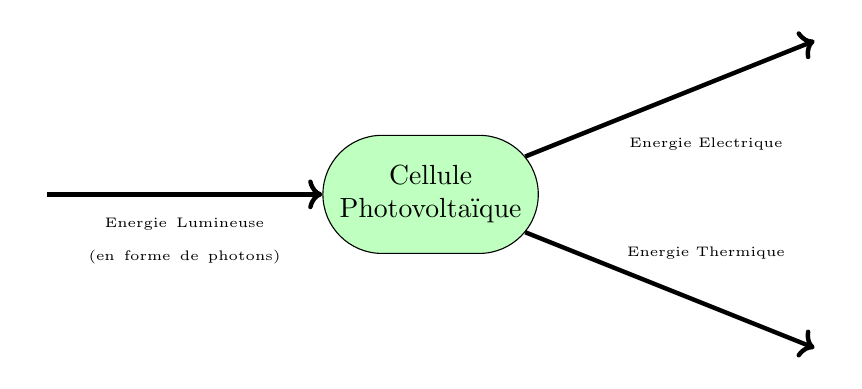
\begin{tikzpicture}
    \draw (5,0) node(C) [draw,
        fill = white!75!green,
        rounded rectangle,
        minimum height = 1.5cm,
        align = center
    ]
    {Cellule \\ Photovoltaïque};
    \draw (0,0) node(S) {};
    \draw [ultra thick, ->] (S) -- (C) 
        node [midway, label = 
        {[below, text width = 3cm, align = center, yshift=-0.3cm]
        \tiny Energie Lumineuse (en forme de photons) \normalsize}] {};
    \draw (10, 2) node(E) {};
    \draw [ultra thick, ->] (C) -- (E)
        node [midway, label = 
        {[align = center, below, yshift = -0.5cm, xshift = 0.5cm]
        \tiny Energie Electrique \normalsize}]{};
    \draw (10, -2) node(H) {};
    \draw [ultra thick, ->] (C) -- (H)
    node[midway, label = {[align = center, above, yshift = 0.1cm, xshift = 0.5cm]
    \tiny Energie Thermique \normalsize}] {};
\end{tikzpicture}
\end{center}

\subsubsection*{1.7. Une cellule photovoltaïque est-elle un récepteur ou un génerateur électrique?}

Une cellule photovoltaïque est un génerateur électrique.

\newpage
\section{Determination du Rendement d'une Cellule Photovoltaïque}
\subsubsection*{2.1 Proposer un protocole experimental afin de déterminer la puissance 
maximale de la cellule photovoltaïque en précisant:}

\begin{itemize}
    \item les paramètres à fixer
    \item les grandeurs à mesurer
    \item l'exploitation des mesures
    \item le schéma du montage expérimental
\end{itemize}


Le materiel necessaire est: une lampe, une cellule photovoltaique, une resistance
variable, deux multimètres, 5 fils electriques au minimum et un tableur. 
\begin{enumerate}
    \item Mettre en place un circuit électrique qui permet de mesurer
            l'intensité et la tension d'une cellule photovoltaïque en 
            fonction d'une résistance variable.
    \begin{center}
    \begin{circuitikz}[european]
        \draw (0,0) -- (0,0.5) to[pvsource, *-*] (0,3.5) -- (0,4) 
        -- (3,4) to[vR] (3,2) to[rmeter, t=A] (3,0) -- (0,0);
        \draw (0,0.5) -- (-2, 0.5) to[rmeter, t=V] (-2, 3.5) -- (0,3.5);
    \end{circuitikz}
    \end{center}
    % Insert schema
    \item Dans un tableur, on note les differentes valeurs de l'intensité (en Ampères) et 
            de la tension (en Volts) pour la résistance allant de $0\ \Omega$ a $20\ \Omega$.
    \item On calcule la puissance pour chacune des mesures et on le présente dans un tableau.
            On détermine sur le graphique pour quelle résistance la puissance fournie par
            la cellule photovoltaïque est maximale.
\end{enumerate}

\subsubsection*{2.2 Mettre en œuvre votre protocole expérimental.}

Fait en classe.

\subsubsection*{2.3 Déterminer la puissance maximale de la cellule photovoltaïque à notre
disposition.}

D'après nos mesures, la puissance maximale de $0.00220\ W$ est atteinte pour $R = 4\ \Omega$.

\subsubsection*{2.4 En déduire son rendement et commenter.}
 
Le calcul du rendement est:
\[\eta = \frac{P_{\text{utile}}}{P_{\text{re\c{c}ue}}}\]
On a $P_{\text{utile}} = 0.00220\ W$, on cherche donc à calculer ${P_{\text{re\c{c}ue}}}$.
\\
D'après la formule qui donne la puissance lumineuse:
\[P_{\text{re\c{c}ue}} = E \cdot S\] avec $P_{\text{re\c{c}ue}} \text{ en } W \text{, } E \text{ l'eclairement en } 
W \cdot m^{-2} \text{ et } S \text{ la surface éclairée en } m^2$.
\\
La surface de la cellule photovoltaïque est de $7,1\ cm$ par $4,1\ cm$ donc:
\[7,1 \cdot 10^{-2} \cdot 4,1 \cdot 10^{-2} = 0.002911\ m^2\]
En gardant la même position de lampe, on garde le même éclairement et on trouve: 
 
\[6500\ lux = \frac{6500}{126}\ W\cdot m^{-2} \approx 51,58\ W \cdot m^{-2}\]
Ce qui donne:

\[P_{\text{re\c{c}ue}} = 51,58 \cdot 0,0029 = 0,1496\ W\]
Donc:
\[ \eta = \frac{P_{\text{utile}}}{P_{\text{re\c{c}ue}}} = \frac{0,00220}{0,1496} = 0,147 = 14,7\%\]

\subsubsection*{2.5 Evaluer l'ordre de grandeur de la puissance maximale fournie par le "champ" de cellules 
photovoltaïques représentées par un carré blanc sur la photographie. On
fera l'hypothèse que les cellules et l'éclairement sont les mêmes que dans l'expérience.}
 
L'échelle sur la photographie est de $1\ cm \longleftrightarrow 1\ km$ et on mesure 
le carre blanc qui a un côté de $1,4\ cm \longleftrightarrow 1,4\ km$ donc l'aire est
de :
\[\mathcal{A}_{\text{carré blanc}} = 1,4 \cdot 10^3 \cdot 1,4 \cdot 10^3 = 1\ 960\ 000\ m^2\]
D'après l'énoncé, les conditions d'éclairage et de résistance sont identique 
à l'expérience effectuée auparavant donc l'éclairement est de $51,58\ W\cdot m^{-2}$
donc :
\[P_{\text{re\c{c}ue}} = 51,58 \cdot 1\ 960\ 000 = 101\ 096\ 800\ W\]
De plus, puisque
$\eta = \frac{P_{\text{utile}}}{P_{\text{re\c{c}ue}}}$,
\\
Alors :
\[P_{\text{utile}} = P_{\text{re\c{c}ue}} \cdot \  \eta = 
101\ 096\ 800\cdot 0,147 = 14\ 861\ 229\ W \approx 14,86\ MW\]
\\
L'aire colorié en blanc dans la photographie produit environ $14,86\ MW$ si l'on
a les mêmes conditions que dans l'expérience.


\end{document}
